\documentclass[11pt]{article}
\usepackage[margin=1in]{geometry}
\usepackage{tikz}
\usetikzlibrary{arrows.meta, positioning, calc, fit, backgrounds}
\usepackage{amsmath, amssymb}
\usepackage{booktabs}
\usepackage{hyperref}
\usepackage{xcolor}

\definecolor{proj}{HTML}{4A90D9}
\definecolor{up}{HTML}{7BC67E}
\definecolor{conv}{HTML}{E8A838}
\definecolor{act}{HTML}{D95B5B}
\definecolor{bg}{HTML}{F5F5F5}

\title{\textbf{Hydro Model Architectures}}
\author{autopath}
\date{}

\begin{document}
\maketitle
\thispagestyle{empty}

\section{Overview}

The \texttt{Hydro} datablock provides a flexible framework for latent-to-image decoders. It is designed to invert feature extractors (e.g., GigaPath) by mapping their embeddings back to the original image space. The system supports multiple architectural versions, dispatched via the \texttt{version} parameter in the model configuration.

\section{Model\_0: Deconvolutional Decoder}

\texttt{Model\_0} is the baseline architecture, using progressive upsampling via transposed convolutions or bilinear interpolation to reconstruct $N \times N$ RGB images from $K$-dimensional latent vectors.

\begin{center}
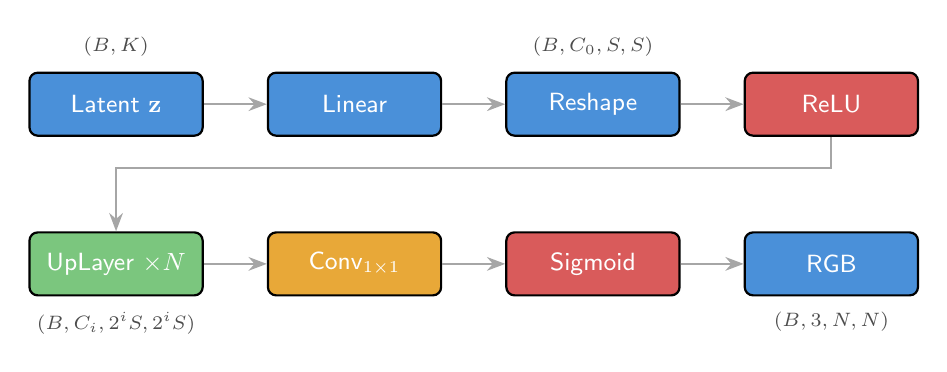
\begin{tikzpicture}[
    >=Stealth,
    block/.style={draw, rounded corners=3pt, minimum height=0.8cm, minimum width=2.2cm,
                  font=\small\sffamily, thick, text=white},
    arrow/.style={->, thick, color=gray!70},
    label/.style={font=\scriptsize\sffamily, color=gray!60!black},
]
    % Row 1: Projection
    \node[block, fill=proj] (input) {Latent $\mathbf{z}$};
    \node[block, fill=proj, right=0.8cm of input] (linear) {Linear};
    \node[block, fill=proj, right=0.8cm of linear] (reshape) {Reshape};
    \node[block, fill=act, right=0.8cm of reshape] (relu) {ReLU};

    % Row 2: Upsampling & Output
    \node[block, fill=up, below=1.2cm of input] (up) {UpLayer $\times N$};
    \node[block, fill=conv, right=0.8cm of up] (final) {Conv$_{1\times1}$};
    \node[block, fill=act, right=0.8cm of final] (sigmoid) {Sigmoid};
    \node[block, fill=proj, right=0.8cm of sigmoid] (output) {RGB};

    % Arrows
    \draw[arrow] (input) -- (linear);
    \draw[arrow] (linear) -- (reshape);
    \draw[arrow] (reshape) -- (relu);
    
    % Connection between rows
    \draw[arrow] (relu.south) -- ++(0,-0.4) -| (up.north);

    \draw[arrow] (up) -- (final);
    \draw[arrow] (final) -- (sigmoid);
    \draw[arrow] (sigmoid) -- (output);

    % Dimension labels
    \node[label, above=2pt of input] {$(B, K)$};
    \node[label, above=2pt of reshape] {$(B, C_0, S, S)$};
    \node[label, below=2pt of up] {$(B, C_i, 2^iS, 2^iS)$};
    \node[label, below=2pt of output] {$(B, 3, N, N)$};
\end{tikzpicture}
\end{center}

\subsection{Architecture Details}

\subsubsection{Initial Projection}
The latent vector $\mathbf{z} \in \mathbb{R}^K$ is projected to a spatial feature map:
\[
    \mathbf{z} \xrightarrow{\text{Linear}} \mathbb{R}^{C_0 \cdot S^2}
    \xrightarrow{\text{Reshape}} \mathbb{R}^{C_0 \times S \times S}
    \xrightarrow{\text{ReLU}} \mathbf{F}_0
\]
where $S$ is the \texttt{initial\_size} (default 8) and $C_0 = H \cdot m_0$ with $H$ = \texttt{hidden\_channels} and $m_0$ the first channel multiplier.

\subsubsection{Progressive Upsampling}
The number of upsample layers is $N_{\text{up}} = \log_2(N / S)$. Each \texttt{UpLayer} doubles spatial resolution:

\begin{center}
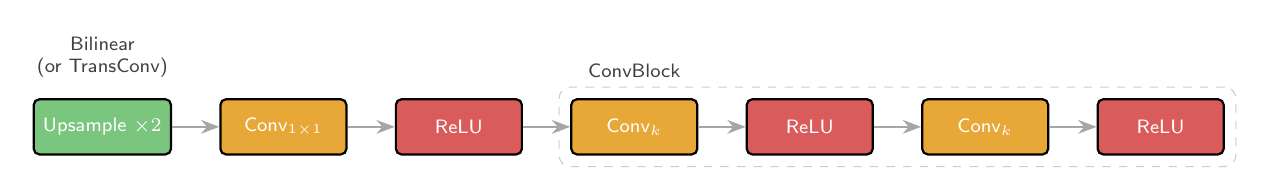
\begin{tikzpicture}[
    >=Stealth,
    block/.style={draw, rounded corners=2pt, minimum height=0.7cm, minimum width=1.6cm,
                  font=\scriptsize\sffamily, thick, text=white},
    arrow/.style={->, thick, color=gray!70},
    label/.style={font=\scriptsize\sffamily, color=gray!50!black, align=center},
]
    \node[block, fill=up] (upsample) {Upsample $\times2$};
    \node[block, fill=conv, right=0.6cm of upsample] (conv1x1) {Conv$_{1\times1}$};
    \node[block, fill=act, right=0.6cm of conv1x1] (relu1) {ReLU};
    \node[block, fill=conv, right=0.6cm of relu1] (conv3a) {Conv$_{k}$};
    \node[block, fill=act, right=0.6cm of conv3a] (relu2) {ReLU};
    \node[block, fill=conv, right=0.6cm of relu2] (conv3b) {Conv$_{k}$};
    \node[block, fill=act, right=0.6cm of conv3b] (relu3) {ReLU};

    \draw[arrow] (upsample) -- (conv1x1);
    \draw[arrow] (conv1x1) -- (relu1);
    \draw[arrow] (relu1) -- (conv3a);
    \draw[arrow] (conv3a) -- (relu2);
    \draw[arrow] (relu2) -- (conv3b);
    \draw[arrow] (conv3b) -- (relu3);

    % Labels
    \node[label, above=4pt of upsample] {Bilinear\\(or TransConv)};
    \node[label, above=4pt of conv3a] {ConvBlock};

    % Brace for ConvBlock
    \begin{scope}[on background layer]
        \node[draw=gray!40, dashed, rounded corners=4pt,
              fit=(conv3a)(relu3), inner sep=4pt] {};
    \end{scope}
\end{tikzpicture}
\end{center}

Two upsampling modes are available, controlled by \texttt{use\_bilinear\_upsampling}:
\begin{itemize}
    \item \textbf{Bilinear} (default): bilinear interpolation $\times2$ followed by $1\times1$ conv + ReLU.
    \item \textbf{Transposed convolution}: \texttt{ConvTranspose2d} with $2\times2$ kernel and stride 2.
\end{itemize}

\subsubsection{Output Head}
A $1\times1$ convolution maps the final feature channels to 3 (RGB), followed by sigmoid activation and scaling:
\[
    \mathbf{I} = \text{sigmoid}\!\big(\text{Conv}_{1\times1}(\mathbf{F}_{N_\text{up}})\big) \times 255
\]

\subsection{Tensor Dimensions (Default Config)}
With $K=1536$, $N=256$, $S=8$, $H=256$, multipliers $(8,4,2,1,1)$:

\begin{center}
\small
\begin{tabular}{lccc}
\toprule
\textbf{Stage} & \textbf{Channels} & \textbf{Spatial} & \textbf{Tensor Shape} \\
\midrule
Input latent     & ---  & --- & $(B, 1536)$ \\
After projection & 2048 & $8$  & $(B, 2048, 8, 8)$ \\
UpLayer 0        & 2048 & $16$ & $(B, 2048, 16, 16)$ \\
UpLayer 1        & 1024 & $32$ & $(B, 1024, 32, 32)$ \\
UpLayer 2        & 512  & $64$ & $(B, 512, 64, 64)$ \\
UpLayer 3        & 256  & $128$ & $(B, 256, 128, 128)$ \\
UpLayer 4        & 256  & $256$ & $(B, 256, 256, 256)$ \\
Final conv       & 3    & $256$ & $(B, 3, 256, 256)$ \\
\bottomrule
\end{tabular}
\end{center}

\section{System Configuration}

The \texttt{Hydro} datablock uses a shared configuration dataclass to control architecture and training parameters.

\begin{center}
\begin{tabular}{lll}
\toprule
\textbf{Parameter} & \textbf{Default} & \textbf{Description} \\
\midrule
\texttt{latent\_dim} & 1536 & Input latent vector dimension $K$ \\
\texttt{image\_size} & 256 & Output resolution $N \times N$ \\
\texttt{initial\_size} & 8 & Spatial size before upsampling \\
\texttt{hidden\_channels} & 256 & Base channel count $H$ \\
\texttt{channel\_multipliers} & $(8,4,2,1,1)$ & Per-layer channel multiplier \\
\texttt{kernel\_size} & 3 & Convolution kernel size \\
\texttt{use\_batch\_norm} & True & BatchNorm in conv blocks \\
\texttt{use\_bilinear\_upsampling} & True & Bilinear vs.\ transposed conv \\
\texttt{loss\_type} & \texttt{mse} & MSE, L1, or L0 reconstruction loss \\
\texttt{version} & 0 & Model architecture version \\
\bottomrule
\end{tabular}
\end{center}

\section{Loss Functions}

The following reconstruction losses are supported:
\[
    \mathcal{L} = \begin{cases}
        \frac{1}{3N^2}\|\hat{\mathbf{I}} - \mathbf{I}^*\|_2^2 & \text{if \texttt{loss\_type} = ``mse''} \\[4pt]
        \frac{1}{3N^2}\|\hat{\mathbf{I}} - \mathbf{I}^*\|_1   & \text{if \texttt{loss\_type} = ``l1''} \\[4pt]
        \frac{1}{3N^2} \sum \log(1 + \frac{(\hat{\mathbf{I}} - \mathbf{I}^*)^2}{\epsilon}) & \text{if \texttt{loss\_type} = ``l0''}
    \end{cases}
\]
where $\epsilon = 10^{-3}$ and $\mathbf{I}^* \in [0, 255]^{3 \times N \times N}$.

\end{document}
